\documentclass[english]{article}

%\usepackage[T1]{fontenc}
\usepackage[latin9]{inputenc}
\usepackage[letterpaper]{geometry}
\geometry{verbose,tmargin=1in,bmargin=1in,lmargin=1in,rmargin=1in}
\usepackage{babel}
\usepackage{amsmath}
\usepackage{amssymb}
\usepackage{capt-of}
\usepackage{graphicx}
\usepackage[usenames,dvipsnames]{color}
\usepackage{latexsym}
\usepackage{xspace}
\usepackage{pdflscape}
\usepackage[hyphens]{url}
\usepackage[colorlinks]{hyperref}
\usepackage{enumerate}
\usepackage{ifthen}
\usepackage{float}
\usepackage{array}
\usepackage{tikz}
\usetikzlibrary{shapes}
\usepackage{algorithm2e}

%%%% HW instructions / collaboration text

\newcommand{\HWPolicies}{
\paragraph*{Instructions.} 

\paragraph*{Collaboration.} 
You are allowed and encouraged to work together. You may discuss the
homework to understand the problem and reach a solution in groups up
to size {\bf four students.} However, {\em each student must write
  down the solution independently, and without referring to written
  notes from the joint session. {\bf In addition, each student must
    write on the problem set the set of people with whom s/he
    collaborated.}} You must understand the solution well enough in
order to reconstruct it by yourself. (This is for your own benefit:
you have to take the exams alone.)
}

\newcommand{\ProgrammingPolicies}[1]{
\paragraph*{Instructions.}

\paragraph*{Collaboration.} 
For this programming assignment, you are {\bf not} allowed to
collaborate with other students. You may {\em discuss} the homework to
understand the problem, but {\bf you are not allowed to share your
code with any other students.} We will be using automatic checking
software to detect blatant copying of other student's assignments, so,
please, don't do it.
}

%%%% CUSTOM COMMANDS FOR FORMATTING EXAMS/HOMEWORKS
\newcounter{section_points}[section]
\newcounter{header_points}[section]
\newcounter{total_points}

\newcommand{\hpoints}[1]{
  \setcounter{header_points}{#1}
  \textbf{[#1 points]}
}

\newcommand{\points}[1]{
  \addtocounter{section_points}{#1}
  \addtocounter{total_points}{#1}
  \textbf{[#1 
    \ifthenelse{\equal{#1}{1}}
    {point}{points}]}
}

\newcommand{\point}{\textbf{[1 point]}}

\newboolean{ShowSolutions}
\newcommand{\Mistake}[2]{
  \ifthenelse{\boolean{ShowSolutions}}
  {\paragraph{\bf $\blacksquare$ COMMON MISTAKE #1:} {\sf #2} \bigskip}
  {}
}

\newcommand{\Solution}[2]{
  \ifthenelse{\boolean{ShowSolutions}}
    {
      \paragraph{\bf $\bigstar $ SOLUTION:} { \sf
        #1} \bigskip
    }
    { 
      #2
    } %} \vspace{1.5in}}
}
\newcommand{\out}[1]{}

\newboolean{ShowPointsInfo}

\newcommand{\PointStats}[0]{
  \ifthenelse{\boolean{ShowPointsInfo}}
  {
    \begin{center}

      \begin{tabular}{rl}
        \hline
        Stated Points: & \arabic{header_points} \\
        Section Points: & \arabic{section_points} \\
        Total Points So Far: & \arabic{total_points} \\
        \hline 
        \multicolumn{2}{c}{
          
          \ifthenelse{
            \equal{\value{section_points}}{\value{header_points}}
          }{CORRECT TOTAL}
          {{\bf INCORRECT TOTAL}}
          }
          \\
        \hline
      \end{tabular}
    \end{center}
  }{}
}

\newcounter{blankcount}
\newcommand{\myrepeat}[2] {
\setcounter{blankcount}{1}
\whiledo{\value{blankcount} < #1}{
#2
\addtocounter{blankcount}{1}
}
}

\newcommand{\blank}[1]{\underline{\myrepeat{#1}{\qquad}}}


%%%% CUSTOM MATH GOES HERE

\newcommand{\ind}[1]{\mathbf{1}\left(#1\right)}
\renewcommand{\Pr}{\mathbf{Pr}\xspace}
\newcommand{\Bern}{\textsf{Bernoulli}\xspace}
\newcommand{\sign}{\textsf{sign}}

\newcommand{\E}{\mathbf{E}}
\newcommand{\bx}{\mathbf{x}}
\newcommand{\bz}{\mathbf{z}}
\newcommand{\bw}{\mathbf{w}}
\newcommand{\bl}{\mathbf{\ell}}
\newcommand{\vc}[1]{\mathbf{#1}}

\newcommand{\Hypo}{\mathcal{H}}
\newcommand{\XX}{\mathcal{X}}
\newcommand{\cD}{\mathcal{D}}


% CIS580 packages
\usepackage{subfigure}
\usepackage{rotating}
\usepackage{verbatim}
\usepackage{graphicx}
% CIS580 notations
\newcommand{\R}{\mathbb{R}}
\newcommand{\Z}{\mathbb{Z}}
\newcommand{\C}{\mathbb{C}}

\usepackage{txfonts}
\newcommand{\ra}{\rightarrow}
\newcommand{\rect}{\text{rect}}
\newcommand{\F}{\mathcal{F}}
\newcommand{\w}{\omega}
\newcommand{\s}{\sigma}
\newcommand{\intinf}{\int_{-\infty}^{\infty}}
\newcommand{\suminf}{\sum_{n=-\infty}^{\infty}}
\newcommand{\fmap}{\multimapdotbothA}
\newcommand{\fmapvert}{\multimapdotbothAvert}

\newcommand{\ds}{\displaystyle}

% Vectors and matrices
\newcommand{\mat}[2]{
  \left[\begin{array}{#1} #2\end{array}\right]
}


% Dirac comb
\input cyracc.def
\font\tencyr=wncyr10
\def\cyr{\tencyr\cyracc}
\def\comb{\mbox{\cyr SH}}

\newcolumntype{M}{>{$\vcenter\bgroup\hbox\bgroup}c<{\egroup\egroup$}}


% COMMAND TO INSERT MATLAB LISTING
% Example
% \matlabscript{ocr/runHomework}{Script generating answers}

\usepackage{listings}
% This is the color used for MATLAB comments below
\definecolor{MyDarkGreen}{rgb}{0.0,0.4,0.0}

% For faster processing, load Matlab syntax for listings
\lstloadlanguages{Matlab}%
\lstset{language=Matlab,                        % Use MATLAB
        frame=single,                           % Single frame around code
        basicstyle=\scriptsize\ttfamily,             % Use small true type font
        keywordstyle=[1]\color{Blue}\bf,        % MATLAB functions bold and blue
        keywordstyle=[2]\color{Purple},         % MATLAB function arguments purple
        keywordstyle=[3]\color{Blue}\underbar,  % User functions underlined and blue
        identifierstyle=,                       % Nothing special about identifiers
                                                % Comments small dark green courier
        commentstyle=\usefont{T1}{pcr}{m}{sl}\color{MyDarkGreen}\scriptsize,
        stringstyle=\color{Purple},             % Strings are purple
        showstringspaces=false,                 % Don't put marks in string spaces
        tabsize=5,                              % 5 spaces per tab
        %
        %%% Put standard MATLAB functions not included in the default
        %%% language here
        morekeywords={xlim,ylim,var,alpha,factorial,poissrnd,normpdf,normcdf},
        %
        %%% Put MATLAB function parameters here
        morekeywords=[2]{on, off, interp},
        %
        %%% Put user defined functions here
        morekeywords=[3]{FindESS, homework_example},
        %
        morecomment=[l][\color{Blue}]{...},     % Line continuation (...) like blue comment
        numbers=left,                           % Line numbers on left
        firstnumber=1,                          % Line numbers start with line 1
        numberstyle=\scriptsize\color{Blue},    % Line numbers are blue
        stepnumber=5                            % Line numbers go in steps of 5
        }

\newcommand{\matlabscript}[2]
  {\begin{itemize}\item[]\lstinputlisting[caption=#2,label=#1]{#1.m}\end{itemize}}



%% WHETHER OR NOT SOLUTIONS ARE ENABLED %%
\setboolean{ShowSolutions}{true}

\title{CIS 580, Machine Perception, Spring 2018: Assignment 3
\ifthenelse{\boolean{ShowSolutions}}{ \\ \bf Solutions }{} }
\date{}

\begin{document}
\maketitle

\begin{itemize}
\item This is an individual homework.% and is worth 100 points.
\item You must submit your solutions online on \href{https://gradescope.com/courses/14413}{Gradescope}, the entry code for which is MKYGP8. We recommend that you use \LaTeX, but we will accept scanned solutions as well.
\item The following files must be submitted via turnin: \verb|gaussian1d.m|, \verb|gaussian2d.m|, \verb|gaborFilter1D.m|,  \verb|gaborFilter2D.m|, \verb|dog1d.m|.
  We provide a few tests; use \verb|run test/run_tests| to run them.
  Please make sure that the given tests are passing before submitting your work.
\item Start early! If you get stuck, please post your questions on \href{https://piazza.com/class/jcamop0erj15o0}{Piazza} or come to office hours!
\end{itemize}

\vspace{1cm}
\section{Gabor filters}
In this section, we will implement 2D detection using a Gabor filter. We will first play with two toy examples in 1D and 2D to understand the fundamentals, then we will attempt to have your computer play the game of ``Where's Waldo''.


\begin{enumerate}
\item \textbf{Gabor filter in 1D}

  In this question we will consider the script \verb!gabor1d_script.m! in the homework kit: it generates a 1D signal of increasing frequency \verb!s! as well as a vector \verb!s_w! containing ground-truth frequencies (see figure \ref{incr_freq}).
  \begin{figure}[ht!]
    \begin{center}
      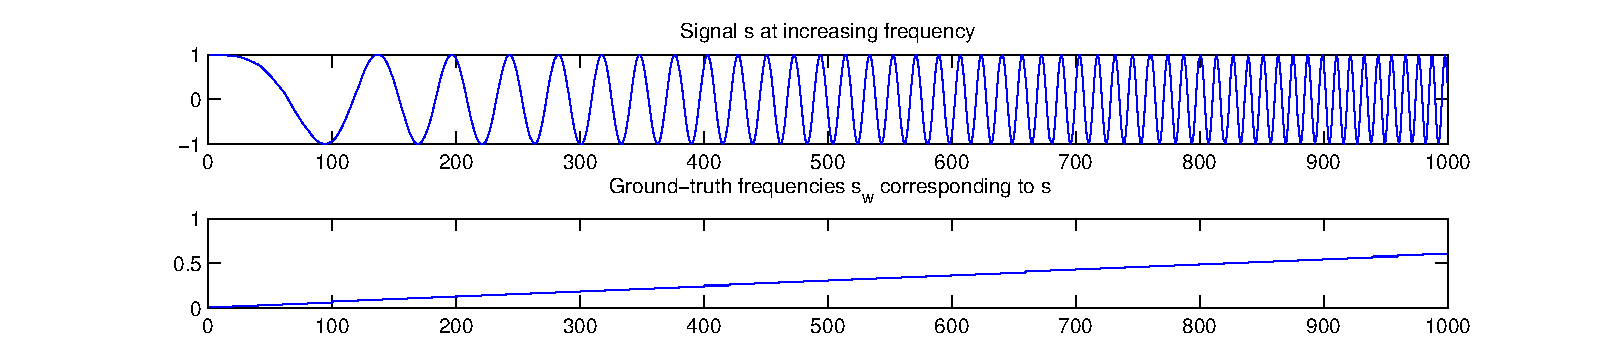
\includegraphics[width = \textwidth]{images/incr_freq_signal.pdf}
    \end{center}
    \caption{\label{incr_freq} Signal at increasing frequencies and corresponding ground-truth frequencies.}
  \end{figure}

  \begin{enumerate}
  \item \points{1} Complete the function \verb!gaussian1d.m! that returns discrete normalized centered Gaussian of given standard deviation $\sigma$ and length.
  \item \points{2} Complete the function \verb!gaborFilter1D.m! that returns a pair of Gabor quadrature filters at given spatial period \verb!T_f! in pixels, Gaussian envelope $\sigma$ and length. The two filters correspond respectively to the real and imaginary part of the Gabor filter we defined in class.
  \item \points{4} Complete the script \verb!gabor1d_script.m! to compute the filter response: \verb!r1!, \verb!r2! are the imaginary and real parts of the response, and \verb!energy! is the magnitude of the response (complex norm).
  \item \points{2} Using the script, plot figures for two distinct values of $T_f$ and check that the maximum response matches the ground truth.
  \end{enumerate}

\item \textbf{Gabor filter in 2D}

  We now consider the same problem in 2D: we want to detect patterns with a specific spatial period \emph{and} orientation in the image represented in figure \ref{incr_freq_2d}.
    \begin{figure}[ht!]
    \begin{center}
      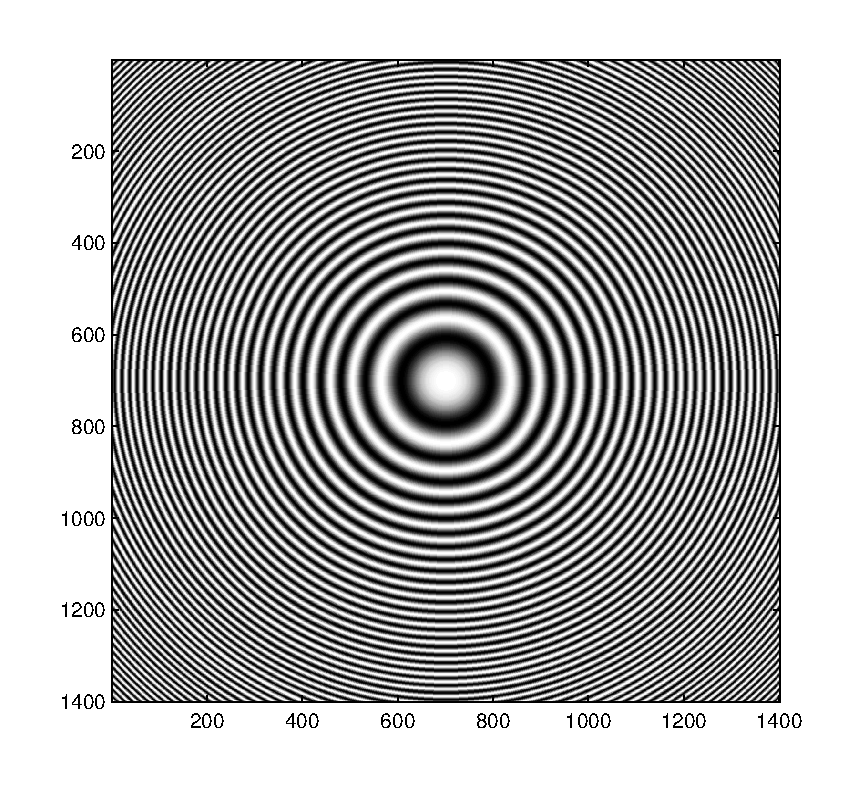
\includegraphics[width = 0.5\textwidth]{images/incr_freq_2d.pdf}
    \end{center}
    \caption{\label{incr_freq_2d} Image containing a range of frequencies and orientations.}
  \end{figure}

  \begin{enumerate}
  \item \points{2} Complete the function \verb!gaussian2d.m! that returns discrete normalized centered 2D Gaussian of given covariance matrix $\Sigma$ and size.
  \item \points{5} Complete the function \verb!gaborFilter2D.m! that returns a pair of Gabor quadrature filters to detect a given spatial period \verb!T_f! in pixels \textbf{and} orientation \verb!theta! in degrees. The two filters correspond respectively to the real and imaginary part of the Gabor filter we defined in class. 
  \item \points{4} Complete the script \verb!gabor2d_script.m! to compute the filter response: \verb!r1!, \verb!r2! are the imaginary and real parts of the response, and \verb!energy! is the magnitude of the response (complex norm).
  \item \points{2} Using the script, plot figures for two distinct values of $T_f$ and check that the maximum response matches the ground truth.
  \end{enumerate}

\item \textbf{Where's Waldo?}

  Now we consider the classical game of finding Waldo (a character with a red-and-white striped shirt) in an image like figure \ref{im:waldo}. We are going to use the function \verb!gaborFilter2D! to craft a filter for horizontal oscillation at an appropriate frequency.
  \begin{figure}[ht!]
    \begin{center}
      
\includegraphics[width = 0.5\textwidth]{images/waldo.jpg}
    \end{center}
    \caption{\label{im:waldo} Where's Waldo?}
  \end{figure}
  
  \begin{enumerate}
  \item \points{2} Read through the script \verb!waldo_script.m! and describe what it does in a couple sentences.
  \item \points{2} Look at the first plot (run the script up to line 28 included) and explain in a few words the formula for \verb!im_red!, line 14.
  \item \points{6} Complete the function \verb!determineStripePeriod.m! that interactively determines the spatial frequency of Waldo-like stripes in the image: you only need to complete the part computing \verb!T_y! after the user clicks on a peak of the fft.
  \item \points{8} Complete end of the script \verb!waldo_script.m! to compute the response of the Gabor filter and the detection mask: figure \ref{waldo_example} shows a part of the image multiplied by \verb!detection_mask!, which is a double matrix equal to $1$ in the candidate areas and $0$ anywhere else.

    You can compute \verb!detection_mask! by thresholding \verb!energy! and by applying \verb!imdilate! with a \verb!'disk'! structuring element of size $30$, to make the zones slightly bigger and include a small portion of the image around the detected stripes: it makes it more convenient to see Waldo's head! Read the documentation of \verb!imdilate! and \verb!strel! for more details.
    \begin{figure}[ht!]
      \begin{center}
        \includegraphics[width = 0.5\textwidth]{images/waldo_example_output.png}
      \end{center}
      \caption{\label{waldo_example} Example output: the energy response is thresholded and dilated, and the resulting detection mask is applied to the image to show only candidate zones with stripes at the right frequency. }
    \end{figure}
  \end{enumerate}
\end{enumerate}



%%% Local Variables: 
%%% mode: latex
%%% TeX-master: "../hw3"
%%% End: 

\clearpage
\section{AlexNet}

\href{http://papers.nips.cc/paper/4824-imagenet-classification-with-deep-convolutional-neural-networks.pdf}{AlexNet}
\footnote{Krizhevsky, A., Sutskever, I., Hinton, G. E. (2012). Imagenet classification with deep convolutional neural networks. In Advances in neural information processing systems (pp. 1097-1105).}  popularized convolutional neural networks (CNNs) after winning the \href{http://image-net.org/challenges/LSVRC/2012/index}{ImageNet ILSVRC 2012} challenge with a huge margin to the runner-up.
It has been observed that the filters in the first layer of a CNN usually resemble Gabor filters.
This question explores this idea.

\begin{enumerate}
\item \points{5} \textbf{Weight visualization}

  Download the pre-trained AlexNet weights here:  \url{http://www.vlfeat.org/matconvnet/models/imagenet-caffe-alex.mat}.
  Load the weights of the first layer on MATLAB by doing:
  \begin{lstlisting}[language=matlab]
    model = load('imagenet-caffe-alex.mat');
    weights = model.layers{1}.weights{1};
  \end{lstlisting}
  You should obtain a $11\times 11\times 3\times 96$ tensor.
  This corresponds to 96 filters with dimensions $11\times 11$ and 3 channels (B, G, R).
  Plot the filters arranged in a $12\times 8$ grid. \emph{Hint: normalize the filters to be between 0 and 1 for better visualization.}

  Select, from the 96 filters, examples of filters that can and that cannot be approximated with the real part of a 2D Gabor (as produced by \verb|gaborFilter2D.m|).
  Explain your answer.

  Note that, since the filters are applied convolutionally, we don't care much about the spatial position, i.e., an off-centered filtered with small support is equivalent to its centered version.

\item \points{7} \textbf{Approximating filters with Gabors}
    \begin{figure}[ht!]
      \begin{center}
        
\includegraphics[width=0.4\textwidth]{images/alexnet.png}
      \end{center}
      \caption{\label{fig:alexnet} A couple of AlexNet filters.}
    \end{figure}

  Consider the two filters from Figure~\ref{fig:alexnet}.
  Approximate them by $11\times 11$ 2D Gabor filters.
  Show your approximations and the parameters chosen.

  In AlexNet, each of the $11\times 11\times 3\times 96$ weights of the first layer have to be learned.
  If we were the replace the first layer of AlexNet with a bank of $96$ Gabor filters, how many parameters would have to be learned?
\end{enumerate}



%%% Local Variables: 
%%% mode: latex
%%% TeX-master: "../hw3"
%%% End: 

\clearpage
\section{Scale invariant detection}
In this section, we will implement a scale-invariant blob detector that produces results as in figure \ref{blob_detection}: we will recursively apply a DoG filter to the initial image to build a 3D-matrix of responses, and we will then find local maxima in position and scale. 

\begin{figure}[ht!]
  \begin{center}
    \includegraphics[width = \textwidth]{images/blob_detection.pdf}
  \end{center}
  \caption{\label{blob_detection} Scale-invariant blob detection example.}
\end{figure}


\begin{enumerate}
\item \textbf{Approximating a LoG by a DoG}

  In this section we will experiment with approximating a Laplacian of Gaussian filter by a Difference of Gaussians. To build the intuition we will reason in 1D, i.e\ with a section of the filter. %The only file you need to complete and run is \verb!DoG_script.m!.
  \begin{enumerate}
  \item \points{7} We want to compute and plot a LoG filter, as well as its approximation by DoG filters. Remember the following:
  $$\text{LoG}_{\sigma} = \frac{1}{(k-1)\s^2}\text{DoG}_{\sigma},\quad \text{where }\; \text{DoG}_{\sigma} = G_{k\sigma} - G_{\sigma}$$
  
  In \verb!DoG_script.m!, we will try several values of k in \verb!k_range!. Complete \verb!dog1d.m! and \verb!DoG_script.m!. Quickly comment on the plots you obtain.

  \item \points{2} Explain why you could expect the DoG to get closer to the LoG as $k$ tends to 1. (Remark: Note that in practice, when building a scale space using DoG, we prefer using $k=\sqrt{2}$)
  \item \points{2} In practice, when building the scale space, we intentionally forget the normalizing factor $\frac{1}{(k-1)\s^2}$ and just use the differences of Gaussians. Explain why.
  \end{enumerate}

  
\item \textbf{Detecting sunflowers}

  The LoG filter in 2D is a rotationally symmetric version of the 1D filter we worked with in the previous question (the famous ``mexican hat''). Because of its shape, it makes a good blob detector (a blob is a dark patch on light background). We don't know the size of the blobs to detect a priori, so we build a scale space by applying the filter with wider and wider $\s$. In practice we will approximate the LoG by a DoG. We will implement a simple (but inefficient) version where we do not downsample the image when blurring it.


  \begin{enumerate}
\item \textbf{Preliminaries}

  In this section the only file you need to complete and run is \verb!blob_script.m!. Make sure you:
  \begin{itemize}
  \item change the two paths at the beginning of the file: one is for the image, the other for a function \verb!minmaxfilt! used to find local maxima/minima in an $n$-dimensional array.
  \item run \verb!minmaxfilter_install.m! in \verb!MinMaxFilterFolder!, to compile the mex files for your platform. (The homework kit already includes compiled mex files for 64-bit Linux, so you can skip this step if you're using that platform)
  \end{itemize}

  \item \points{7} Complete the part of \verb!blob_script.m! that builds the 3D matrix \verb!scales!. Each slice \verb!scales(:,:,i)! contains the original image, blurred by a simple Gaussian filter of parameter \verb!sigma_i = sigma * k^(i-1)!. 

    \textbf{Important}: we exploit the fact that the 2D Gaussian filter is separable. Instead of convolving the image with a 2D Gaussian, build a 1D Gaussian filter \verb!g_i! (using \verb!gaussian1d.m!), convolve the image with \verb!g_i! and then with \verb!g_i'! (transpose of \verb!g_i!): this has the same effect as convolving with the 2D filter but is more efficient.
  \item \points{7} Complete the part of \verb!blob_script.m! that filters the local maxima in the scale space according to their response. Here we want to keep only points $(x,y,\s)$ that have a response higher than 50\% of the maximum response accross the whole 3D scale space.
  \item \points{3} The radius of a detected blob corresponds to $\sqrt{2}$ times the detected scale: complete the formula for the radius \verb!r! of each detection, at the end of \verb!blob_script.m!, in order to plot the detections as circles of detected radius on top of the image. \verb!r! depends on \verb!sigma!, \verb!k!, and the detected scale (use \verb!smax!).
  \item \points{7} Show your detection results for the image \verb!sunflowers.jpg! and for another image of your choice containing blobs at various scales. Remark: In case you wonder how to detect white blobs on a dark background, take the local minima instead of local maxima.
  \end{enumerate}
  
\end{enumerate}



%%% Local Variables: 
%%% mode: latex
%%% TeX-master: "../hw3"
%%% End: 


\end{document}
